\subsection{Completeness Properties of (TO)HTN Planners}
\label{improv: completeness}
In our presentation on different search algorithms implemented in CrowdHTN we already did a short discussion on the completeness of different algorithms in section \ref{improv: search completeness}. The current section will start with a short recap of our findings, expand them to other planners and will then do an expanded discussion that takes factors like loop detection and restarts into account. \\
Before we dive into the more detailed discussion we want to note that we have seen in section \ref{prelim: tohtn complexity} that there is an upper bound to task network depth where if a plan exists there always exists a plan up to that depth. By limiting our planning to task network expansions with lower depth, we can trivially achieve completeness. This is however of little practical use as this depth bound is exponential in the problem size. As a result, we can expect to run out of memory before hitting this bound. For this reason we do not make use of this bound and as far as we know no other planner does it either. We will now resume a more practical discussion of planner completeness.\\ 
As previously noted, we can split our search algorithms into three main groups:
\begin{itemize}
	\item Algorithms that are complete (BFS, A-star like search)
	\item Algorithms with a chance but no guarantee to find a plan (DFS)
	\item Algorithms which for some domains will never find a plan (heuristic search with pathological cases)
\end{itemize}
\paragraph{Completeness in other planners}
So far we have only classified the different search algorithms present in CrowdHTN. For now we will take a look at other planners, starting with translation-based planners totSAT (\cite{behnke2018totsat}), Tree-REX (\cite{schreiber2019tree}) and Lilotane (\cite{schreiber2021lilotane}). As we have noted in the discussion on planning algorithms in section \ref{prelim: translation based planners}, all three of these planners are based on SAT. Additionally, they all explore the set of potential expansions of the task hierarchy in a layer-by-layer fashion, leading to a BFS-like characteristic in their behavior. As a result, these planners are complete as they are. \\
In contrast to this, we have the space of search-based planners, starting with HyperTensioN \cite{magnaguagno2020hypertension}. For HyperTensioN, the authors themselves note that their inbuilt loop detection mechanism suffers from false-positives with no mechanism to mitigate them \cite{magnaguagno2020hypertension}. It follows that their planner is not complete. If we disabled the loop detection in HyperTensioN we would be left with a planner performing DFS, which would put it in the category of planners which are not complete but still have a chance to solve any instance. \\
PANDA on the other hand is a planner based on heuristic progression search that offers a number of configuration options for both search and loop detection. Regarding search, PANDA offers both a pure heuristic DFS and a weighted A* search taking into account the previous path \cite{holler2020htn}. For loop detection PANDA offers hashing based mechanisms both with and without a fallback to full search node comparison \cite{holler2021loop}. Completeness of the planner varies depending on the chosen configuration. If loop detection is configured to allow for false positives, we expect PANDA to not be complete regardless of search algorithm, as there is no mechanism in place to mitigate their effect. If a loop detection mechanism is chosen which does not have false positives, we expect PANDA to be complete if weighted A* with a weight $w > 0$ is used, as this introduces a BFS-like behavior into the search. This leaves pure heuristic DFS combined with loop detection which does not suffer from false positives. Due to the complex nature of the PANDA heuristic we were unable to construct any pathological case which leads PANDA into an infinite recursion. As heuristics are inherently limited we do assume that such cases exist. We will explore this case and the similar case in CrowdHTN in the following paragraph.

\begin{comment}
-algorithm:
- in A* configuration: has a BFS like characteristic giving us completeness
- in heuristic search configuration: we assume that there exist pathological cases similar to CrowdHTN
- loop detection:
- based on hash only: we loose parts of the search space, no completeness
- hash and comparison fallback: no false positives, this is nice
- the open question: where does PANDA fall if we use heuristic search and loop detection without false positives?

similar to CrowdHTN with our new heuristic. As a result, we expect there to be instances which are impossible to solve. However, PANDA also contains a number of loop detection mechanisms described in \cite{holler2021loop} which in some configurations does not have false positives.
\todo{Something like, we'll discuss the implications in the next paragraph}
\end{comment}

\paragraph{Loop detection and completeness}
\label{improv: loops and completeness}
As we have seen, heuristic search on its own may increase planner performance but comes at the cost of completeness. We will now explore the implications of combining heuristic search with loop detection to see how this changes the overall situation. In this paragraph we are only interested in loop detection mechanisms that do not suffer from false positives as this automatically disqualifies a planner from being complete. Additionally, we argue from the perspective of progression search where each search node is uniquely identified by the combination of open tasks and world state.\\
In general, loops are only a problem in (TO)HTN planning if there exists at least one recursive task. If no such task exists, there exist only a finite and usually small number of possible task network expansions such that we can easily search the full search space. If we do have a recursive task, we can further classify our instances according to how hard it is to deal with. Here we identify three categories:
\begin{itemize}
	\item Tasks which recurse into themselves with no change in the world state
	\item Tasks which recurse into themselves with changes in the world state
	\item Tasks which recurse into themselves while adding more tasks afterwards
\end{itemize}
In all three cases, a task recursing into itself also implies that the set of legal orderings is a subset of the original set of orderings. \\
The first case is the easiest to detect and to fix. If a task recurses into only itself we do not get any changes to the open tasks. As a result, search nodes before and after this recursion are equivalent. They will be detected by loop detection as it is used in PANDA and CrowdHTN and the search will be guided into a better direction. \\
In the second case we have to perform additional work before a loop can be detected. As the set of open tasks stays the same and the world state changes, we do not immediately get equivalent search nodes. However, in an (TO)HTN instance with predicates $\mathcal{Q}$, there are only $2^{|\mathcal{Q}|}$ possible world states. We can easily see that we will recurse at most $2^{|\mathcal{Q}|}$ times before our loop detection activates and we are guided back into still unexplored parts of the search space. In practice we can often obtain a lower bound on the possible number of recursions by looking only at the predicates which occur as effects in the resolution of any tasks present in the task recursion. We see that, while less efficient, our known loop detection mechanisms correctly deal with this case. \\
This leaves us with the third case, where a task does not directly recurse into itself but where the resolution of task $t$ gives rise to a new instance of $t$ as well as additional tasks $t_1, \ldots, t_k$ which are restricted to be resolved after $t$. As a result, once we re-encounter $t$ our open task set has changed. While we were able to limit the number of possible world states for our previous case, this is not possible here, as the number of open tasks and thus the number of sets of open tasks is unbounded. More specifically, loop detection as used in PANDA and CrowdHTN is unable to handle this case. Figure \ref{figure: pathological heuristic loop} provides an example of an instance which would guide our proposed CrowdHTN heuristic into the recursion while not creating loops, as each recursion changes the open tasks by extending the sequence. As mentioned in the previous paragraph, we assume that similar cases can be constructed for other (TO)HTN heuristics.
\begin{figure}
	\caption{Pathological instance for our proposed heuristic that is not caught by loop detection}
	\label{figure: pathological heuristic loop}
	\centering
	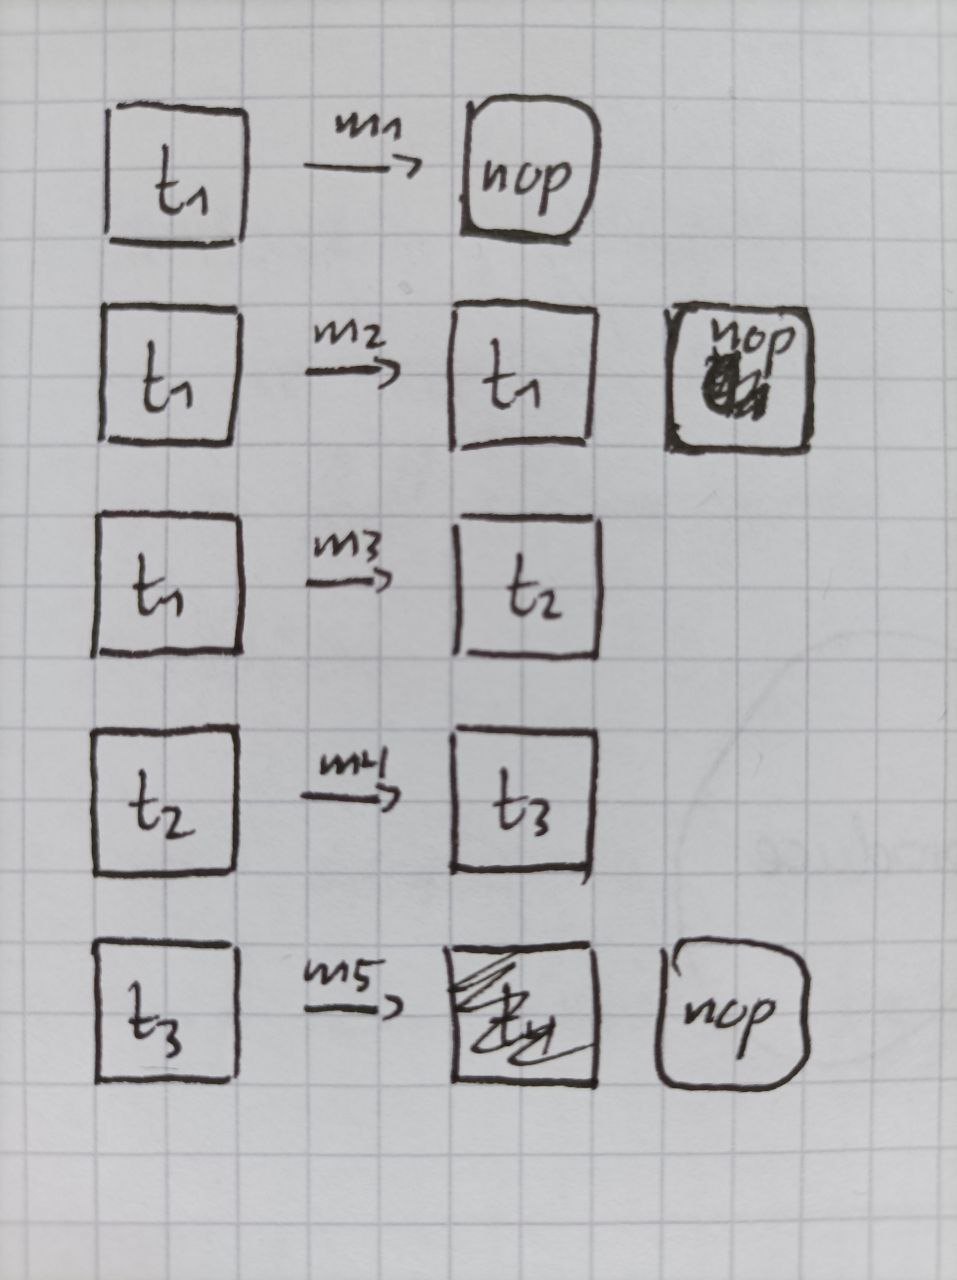
\includegraphics[width=0.3\textwidth]{images/prelim/loop_detection_pathological}
\end{figure}

\paragraph{Restarts and completeness}
So far we have seen that search algorithms with a BFS-like behavior are easily complete. Similarly, we have seen that heuristic search may suffer from pathological cases. This leaves DFS as an open case, where any plan can theoretically be found but not every plan will, due to getting lost in infinite loops. In the previous paragraph we have looked at how loop detection aims to fix this problem and have seen that it does not work for all cases. Now we will look at the restart mechanism we introduced in section \ref{ld - completeness} to mitigate false positives in our approximate loop detection and see how it affects overall completeness. \\
We can make a similar argument as in our previous discussion. In random DFS any path has probability $p > 0$ to be taken. It follows that, as the number of restarts approaches infinity, the probability to take this path at least once approaches 1. This has the additional constraint that we do not only need an unbounded number of restarts but additionally need an unbounded number of runs in between restarts with length at least $t$ for any $t > 0$. Without this constraint we may take the right path but always terminate before we are able to complete it. Our restart mechanism fulfills both of these constraints, using probabilistic restarts with probability $\frac{1}{t}$ after $t$ seconds. With this mechanism, DFS in CrowdHTN gives us a complete planner.

\begin{comment}
- restarts solve the problem for DFS
- but only if we get some additional properties!
- i.e. we expect an infinite number of restarts
- additionally, we get an infinite number of runs longer than $t$ seconds for any $t$

- this is nice and gives completeness (yay!)

- loop detection also helps
- loop detection specifically helps if the wrong path is recursive
- warning: recursive does not just mean that we resolve to the same task
- two cases:
- resolve to same task, but world state is changing
- i.e., we get the exact same open tasks
- or in case of HTN we get the same open tasks and a subset of possible orderings to what we had before
- this will not immediately be detected
- however, the number of possible world states is bound
- so eventually we will find the loop, but it will take time
- resolve to the same task but also add more tasks afterwards ()
- now the open tasks are different and it is not the same search node anymore
- oh, look, an example domain
- the number of open tasks is unbounded
- heuristics cannot be saved via loop detection
- show an example domain with problems! (i.e. search nodes are not identical if we introduce additional open tasks)


- previous section \ref{improv: search completeness} talked about the completeness of different search paradigms

- Lilotane is complete (BFS-like)
- BFS search is complete
- A-star like search is complete

- we could always achieve trivial completeness, but it is not interesting from a practical perspective

- DFS and heuristic search are problematic
- DFS always has a chance to find the right path, but we have to actually hit it
- heuristic search may deterministically take the wrong way
\end{comment}

\paragraph{Conclusion}
In this section we have taken a look at completeness in (TO)HTN planners and how loop detection and restarts can help us to achieve it. We have shown that completeness is highly dependent on the specific search behavior with BFS-like behavior being easiest to turn into a complete planner while heuristic search may always suffer from pathological cases. Additionally, we see that loop detection is able to solve many but not all problems with recursive (TO)HTN instances. In the end, we introduce a restart mechanism and argue that it is able to mitigate problems with false positives in loop detection and allows random DFS to achieve completeness in all cases.

\begin{comment}
- completeness is highly dependent on algorithm
- recursion remains a major challenge
- not only for runtime
- loop detection can fix many of the problems but not all
- instead of only detecting loops we may have to get better at detecting dead ends
- we may want to randomize our heuristics
- keep the benefits
\end{comment}
